\setcounter{chapter}{4}
\chapter{Programación de procesos paralelos con MPI}

\section{Resumen}
En esta práctica se realizó un acercamiento al paradigma de programación paralela distribuida en memoria mediante la interfaz de paso de mensajes \textit{Message Passing Interface} (MPI) e implementación OpenMPI en lenguaje C. Se abordó la configuración del entorno en el sistema operativo GNU/Linux con la instalación de los paquetes \texttt{openmpi-bin}, \texttt{openmpi-dbg} y \texttt{libopenmpi-dev}, así como las reglas de compilación con \texttt{mpicc} y ejecución con \texttt{mpirun}. En la sección práctica se desarrolló un programa en C donde el proceso maestro (nodo 0) coordina a siete nodos esclavos (nodos 1 al 7), enviando a cada uno una fila de una matriz para calcular distintas operaciones aritméticas y retornar los resultados al maestro para su despliegue en pantalla. La compilación fue gestionada mediante un archivo \texttt{Makefile} para cumplir con los lineamientos de la entrega.

\section{Introducción}
En el cómputo paralelo de memoria distribuida, los nodos de procesamiento no comparten un espacio de direcciones de memoria común, por lo que la cooperación entre procesos depende enteramente del intercambio explícito de mensajes a través de una red de datos. La interfaz MPI (\textit{Message Passing Interface}) es la especificación estándar más extendida para gestionar este flujo de comunicación en clústeres y sistemas de supercómputo.

El objetivo general de esta práctica es realizar aplicaciones con procesos en paralelo utilizando la interfaz de paso de mensajes (MPI) en Lenguaje C sobre Linux. Como objetivos específicos se plantea: (1) investigar las herramientas de instalación, compilación y ejecución de OpenMPI; (2) desarrollar un programa que cree 8 procesos en paralelo (nodo maestro y 7 esclavos) para procesar una matriz de datos; y (3) estructurar un archivo \texttt{Makefile} que garantice una compilación limpia sin errores ni advertencias.

\section{Marco teórico}

\subsection{Message Passing Interface (MPI)}
MPI es una especificación estándar de paso de mensajes desarrollada por el \textit{MPI Forum} para permitir que múltiples procesos independientes cooperen mediante el envío y recepción explícita de datos \cite{mpiforum2021}. En C, la interfaz se proporciona mediante la cabecera \texttt{<mpi.h>}, la cual define funciones fundamentales de inicialización (\texttt{MPI\_Init}), finalización (\texttt{MPI\_Finalize}), identificación de procesos (\texttt{MPI\_Comm\_rank}), tamaño del comunicador (\texttt{MPI\_Comm\_size}) y funciones de transmisión punto a punto (\texttt{MPI\_Send} y \texttt{MPI\_Recv}) \cite{pacheco2011}.

\subsection{Instalación y herramientas de OpenMPI}
En distribuciones GNU/Linux como Ubuntu o Debian, OpenMPI provee los componentes esenciales para el desarrollo y depuración de software paralelo \cite{openmpi2024} mediante tres paquetes principales:
\begin{itemize}
    \item \texttt{openmpi-bin}: Contiene los binarios ejecutables del sistema en tiempo de ejecución, como los lanzadores de procesos \texttt{mpirun} y \texttt{mpiexec}.
    \item \texttt{openmpi-dbg}: Proporciona símbolos de depuración para analizar errores a bajo nivel y realizar rastreos de pila con herramientas como \texttt{gdb}.
    \item \texttt{libopenmpi-dev}: Incluye los archivos de cabecera (\texttt{mpi.h}) y bibliotecas necesarias para compilar y enlazar código fuente C/C++.
\end{itemize}

\subsection{Compilación y ejecución de programas MPI}
El flujo de trabajo en consola para programas MPI en C se compone de dos comandos:
\begin{enumerate}
    \item \textbf{Compilación (\texttt{mpicc}):} Es un wrapper sobre el compilador C (\texttt{gcc}) que incluye automáticamente las rutas de cabeceras y banderas de enlazado de bibliotecas MPI.
    \item \textbf{Ejecución (\texttt{mpirun}):} Es el encargado de crear y coordinar las instancias paralelas del ejecutable. La bandera \texttt{-np} especifica la cantidad de procesos que se ejecutarán concurrentemente.
\end{enumerate}

\section{Desarrollo}

Para cumplir con los requerimientos de la práctica, se diseñó un programa en lenguaje C estructurado bajo un esquema maestro-esclavo con 8 procesos en paralelo.

\subsection{Código C del sistema paralelo}
El nodo 0 actúa como maestro, almacenando una matriz de $7 \times 3$ y enviando cada fila $i-1$ al nodo $i$ ($1 \le i \le 7$) usando \texttt{MPI\_Send}. Cada nodo esclavo recibe su fila mediante \texttt{MPI\_Recv}, ejecuta la operación matemática correspondiente y regresa el resultado flotante al nodo 0.

\begin{lstlisting}[style=C, caption={Implementación del programa con MPI (practica5.c)}]
#include <stdio.h>  
#include <mpi.h>  
#include <math.h>  

int main(int argc, char **argv) {  
    int rank, size;  
    float fila[3];  
    float resultado;  
    MPI_Status estatus;  

    MPI_Init(&argc, &argv);  
    MPI_Comm_rank(MPI_COMM_WORLD, &rank);  
    MPI_Comm_size(MPI_COMM_WORLD, &size);  

    if (size < 8) {  
        if (rank == 0) {  
            printf("PRACTICA CON 8 PROGRAMAS\n");  
        }  
        MPI_Finalize();  
        return 0;  
    }  

    if (rank == 0) {  
        float matriz[7][3] = {  
            {1, 2, 3}, {4, 5, 6}, {7, 8, 9},  
            {9, 6, 3}, {-6, -9, -12}, {5, 10, 15}, {7, 14, 21}  
        };  

        printf("Nodo maestro (0) enviando filas a los nodos esclavos...\n");  

        for (int i = 1; i <= 7; i++) {  
            MPI_Send(matriz[i-1], 3, MPI_FLOAT, i, 0, MPI_COMM_WORLD);  
        }  

        for (int i = 1; i <= 7; i++) {  
            MPI_Recv(&resultado, 1, MPI_FLOAT, i, 1, MPI_COMM_WORLD, &estatus);  
            int origen = estatus.MPI_SOURCE;  
            if (origen == 1) printf("Nodo %d hizo a + b + c = %.2f\n", origen, resultado);  
            if (origen == 2) printf("Nodo %d hizo a - b + c = %.2f\n", origen, resultado);  
            if (origen == 3) printf("Nodo %d hizo a * b * c = %.2f\n", origen, resultado);  
            if (origen == 4) printf("Nodo %d hizo a * (b + c) = %.2f\n", origen, resultado);  
            if (origen == 5) printf("Nodo %d hizo a * b - b * c = %.2f\n", origen, resultado);  
            if (origen == 6) printf("Nodo %d hizo c * (a + b)^2 = %.2f\n", origen, resultado);  
            if (origen == 7) printf("Nodo %d hizo a^2 - b^2 + c^3 = %.2f\n", origen, resultado);  
        }  
    } else {  
        if (rank >= 1 && rank <= 7) {  
            MPI_Recv(fila, 3, MPI_FLOAT, 0, 0, MPI_COMM_WORLD, &estatus);  

            float a = fila[0], b = fila[1], c = fila[2];  

            if (rank == 1) resultado = a + b + c;  
            else if (rank == 2) resultado = a - b + c;  
            else if (rank == 3) resultado = a * b * c;  
            else if (rank == 4) resultado = a * (b + c);  
            else if (rank == 5) resultado = (a * b) - (b * c);  
            else if (rank == 6) resultado = c * pow((a + b), 2);  
            else if (rank == 7) resultado = pow(a, 2) - pow(b, 2) + pow(c, 3);  

            MPI_Send(&resultado, 1, MPI_FLOAT, 0, 1, MPI_COMM_WORLD);  
        }  
    }  

    MPI_Finalize();  
    return 0;  
}
\end{lstlisting}

\subsection{Automatización con Makefile}
Se configuró el archivo \texttt{Makefile} para compilar el código de forma limpia con las librerías matemáticas y el compilador de OpenMPI:

\begin{lstlisting}[language=make, caption={Archivo Makefile de la práctica}]
all: practica5

practica5: practica5.c
    mpicc practica5.c -o practica5 -lm

run:
    mpirun -np 8 ./practica5

clean:
    rm -f practica5
\end{lstlisting}
\graphicspath{{practicas/prac01/figuras/}{practicas/prac02/figuras/}{practicas/prac03/figuras/}{practicas/prac05/figuras/}{img/}}
\subsection{Evidencias de Ejecución}
\begin{figure}[H]
    \centering
    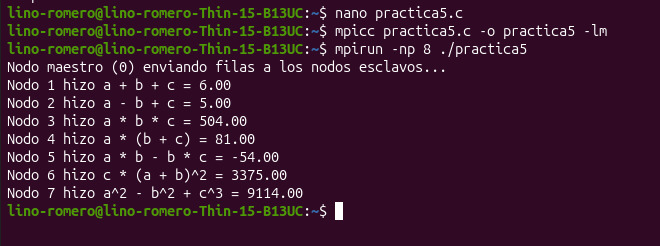
\includegraphics[width=0.75\textwidth]{practicas/prac05/figuras/ejemplo_comando.jpeg}
    \caption{Ejecución del programa paralelo en terminal mediante mpirun con 8 procesos.}
    \label{fig:ejecucion_mpi}
\end{figure}

\section{Conclusiones}
\clearpage
\subsection{Cruz Trejo Said Carbot}
Al concluir esta práctica de programación de cómputo paralelo utilizando la interfaz de paso de mensajes (MPI), me di cuenta del cambio de paradigma tan profundo que exige el diseño de algoritmos concurrentes. A lo largo de mi formación en ingeniería, estuve acostumbrado a diseñar software bajo un modelo estrictamente secuencial, donde el control de flujo de los datos es lineal y predecible. Sin embargo, al implementar OpenMPI en el entorno de desarrollo de macOS, experimenté de primera mano el reto y la ventaja que supone distribuir la carga computacional entre múltiples nodos. 
El desarrollo de los ejercicios iniciales, como el envío de un simple arreglo desde el nodo maestro hacia tres procesos esclavos, fue fundamental para comprender el funcionamiento interno de la comunicación punto a punto en MPI. A través de funciones críticas como MPI\_Send y MPI\_Recv, comprendí que la sincronización de los datos requiere una precisión absoluta en la definición de las etiquetas (tags) y en el manejo del MPI\_Status. 
El desafío principal de esta práctica se presentó al tener que implementar el modelo maestro-esclavo para resolver las operaciones aritméticas de la matriz propuesta. El requerimiento de instanciar exactamente ocho procesos (un maestro y siete esclavos) me obligó a diseñar una topología de comunicación eficiente. En este escenario, el nodo cero tuvo que extraer iterativamente cada fila de la matriz y despacharla al nodo correspondiente. Durante la codificación y la compilación mediante el archivo makefile, me enfrenté al reto de adaptar mi entorno de desarrollo local en macOS para emular el comportamiento de un clúster de procesamiento. La instrucción mpirun -np 8 no solo levantó los procesos, sino que me demostró la verdadera potencia del cómputo paralelo: en un escenario secuencial, calcular las sumas, restas y multiplicaciones de la matriz habría requerido un ciclo for secuencial; en cambio, mediante MPI, los siete cálculos se ejecutaron de manera concurrente. 
Finalmente, esta práctica me permitió consolidar mis conocimientos sobre las operaciones de entrada y salida a bajo nivel en el lenguaje C, así como reafirmar la importancia de la validación estricta de las reglas de negocio establecidas, como evitar el uso de sockets y garantizar que la comunicación se diera exclusivamente por paso de mensajes. Considero que esta experiencia no solo cumple con los objetivos del curso de Cómputo Paralelo, sino que me proporciona una base técnica sumamente robusta para mi futuro desarrollo profesional en inteligencia artificial, un campo donde el entrenamiento de modelos de redes neuronales depende intrínsecamente del procesamiento distribuido y la gestión eficiente de múltiples núcleos. Dominar herramientas como MPI abre la puerta a la optimización de recursos, y comprender su arquitectura a este nivel de detalle ha sido un paso invaluable en mi preparación como ingeniero.

\clearpage
\subsection{López Castro Magaly}
En esta práctica logré consolidar mi comprensión sobre el paradigma de paso de mensajes mediante MPI, comprendiendo que el verdadero poder del supercómputo no radica únicamente en lanzar múltiples procesos al sistema operativo, sino en la orquestación precisa de los mismos. A diferencia de la programación secuencial tradicional, trabajar en un entorno Linux con arquitectura de memoria distribuida me exigió diseñar una estrategia donde el nodo maestro distribuye la carga de trabajo de manera equitativa. Esto es fundamental porque en el campo de la inteligencia artificial y el procesamiento de grandes volúmenes de datos, distribuir las tareas algorítmicas hacia nodos esclavos es la única forma viable de optimizar los tiempos de ejecución y superar los límites físicos del hardware de un solo hilo.

Asimismo, uno de los aprendizajes más valiosos fue dimensionar el impacto que tiene la sobrecarga de comunicación entre los procesos. Entendí que asignar tareas a los nodos requiere una planificación cuidadosa de las primitivas de envío y recepción, asegurando que cada identificador lógico ejecute exclusivamente la subrutina que le corresponde. Si esta sincronización falla o si se envían datos innecesarios a través del comunicador, el tiempo que se pierde en la latencia puede anular por completo la ventaja del paralelismo. Por lo tanto, el reto no solo fue escribir el código en C, sino estructurar las dependencias de los datos para garantizar que las operaciones matemáticas fluyeran hacia el nodo central sin generar cuellos de botella ni bloqueos inesperados.

Por otra parte, la restricción de utilizar un archivo Makefile y mantener una compilación estricta sin advertencias reforzó en mí las buenas prácticas de la ingeniería de software. Al gestionar el proyecto desde la terminal, comprobé que automatizar la construcción del binario con herramientas como mpicc no es un mero requisito de evaluación, sino una práctica indispensable cuando se escalan proyectos a infraestructuras de alto rendimiento. Garantizar un código limpio y validar rigurosamente la correcta recepción de los arreglos en cada nodo esclavo me permitió tener la certeza de que los resultados devueltos al nodo principal eran exactos, previniendo fallos silenciosos que en sistemas concurrentes son extremadamente difíciles de depurar.

Finalmente, esta implementación representó un cambio de mentalidad crucial respecto a la forma en que suelo abordar el diseño de algoritmos. Acostumbrada a buscar la optimización de la complejidad temporal en un solo procesador, adaptar la lógica a un modelo concurrente maestro-esclavo me demostró la importancia de pensar de forma distribuida. En conclusión, esta práctica sentó bases sólidas para mis futuros desarrollos en cómputo paralelo, demostrándome que dominar estándares como MPI es indispensable para diseñar sistemas robustos, aprovechar al máximo las arquitecturas de procesamiento modernas y construir soluciones tecnológicas verdaderamente escalables.
\clearpage
\subsection{Romero Rosales Lino Ehecatl}
En el desarrollo de esta práctica, logré asimilar de manera práctica los fundamentos de la programación paralela a través del estándar MPI. Al principio, la idea de ejecutar múltiples procesos simultáneamente sugería simplemente una mejora automática en la velocidad, pero al implementar el código comprendí que la verdadera complejidad reside en el diseño de la solución. Distribuir las filas de una matriz desde un nodo central hacia varios nodos secundarios me demostró que el paralelismo efectivo requiere una planificación rigurosa. Cada proceso debe tener un propósito bien definido, y en este caso, asignar una operación matemática específica a cada nodo esclavo permitió visualizar cómo se puede fragmentar un problema mayor en unidades de trabajo totalmente independientes.

Otro aspecto fundamental que me dejó esta actividad fue comprender la vital importancia de la comunicación y la sincronización. Implementar el modelo maestro-esclavo me hizo entender que no basta con dividir el trabajo computacional; es indispensable establecer canales de transmisión de datos eficientes. El uso de las funciones de envío y recepción de mensajes implica coordinar los tiempos de ejecución para que el nodo maestro recolecte la información correctamente y los esclavos sepan exactamente cuándo procesar los datos. Si las variables no se envían con las etiquetas adecuadas o si los resultados no se recogen de forma estructurada, el programa puede arrojar resultados erróneos o quedarse bloqueado, lo que me enseñó que el control del flujo de datos es tan crítico como la lógica del algoritmo.

Por otro lado, la exigencia de construir el proyecto utilizando un archivo Makefile y lograr una compilación limpia me ayudó a valorar las herramientas formales de desarrollo de software. Cuando se trabaja con bibliotecas especializadas y comandos de compilación como mpicc, hacerlo de forma manual resulta ineficiente y propenso a equivocaciones. El uso del Makefile automatizó este proceso, garantizando un entorno de pruebas consistente y ordenado. Además, el requisito de no tener errores ni advertencias me hizo adoptar una postura más analítica y disciplinada frente al código, entendiendo que la calidad de un programa paralelo se evalúa desde su correcta construcción estructurada antes de llegar a la fase de ejecución.

A modo de cierre, considero que esta práctica marcó un cambio significativo en mi forma de concebir la resolución de problemas computacionales. Dejar atrás la mentalidad de la programación estrictamente secuencial para adoptar un enfoque distribuido representó un gran desafío. Entender que los recursos de procesamiento pueden aprovecharse al máximo mediante la correcta coordinación de procesos concurrentes me abre un panorama mucho más amplio sobre cómo funcionan los sistemas de alto rendimiento. En conclusión, dominar las bases de MPI y la estructuración de tareas me ha proporcionado una perspectiva valiosa que aplicaré en el futuro al enfrentarme a sistemas que requieran procesar información de manera rápida, eficiente y escalable.
\clearpage
\subsection{Ugalde Téllez Aarón}
En esta práctica pude comprender mejor cómo funciona la programación de procesos paralelos utilizando MPI, ya que al principio puede parecer que ejecutar un programa varias veces es suficiente para aprovechar el procesamiento paralelo, pero en realidad es necesario organizar las tareas y establecer una forma de comunicación entre los procesos. A través de esta práctica entendí que MPI permite dividir el trabajo entre diferentes procesos, de manera que cada uno pueda realizar una parte de las operaciones y posteriormente compartir los resultados cuando sea necesario. Esto es importante porque existen problemas que pueden resolverse de una manera más eficiente cuando se distribuyen las tareas, en lugar de depender de un solo proceso que tenga que realizar todo el trabajo de manera secuencial.

También considero que uno de los aspectos más importantes de esta práctica fue comprender que la programación paralela no consiste solamente en ejecutar varios procesos al mismo tiempo, sino que también es necesario tener cuidado con la manera en que se distribuye el trabajo y se intercambia la información. Por ejemplo, es importante identificar qué proceso se encarga de realizar cada tarea, qué información necesita recibir y qué resultados debe enviar a los demás procesos. De esta manera, se puede evitar que los procesos realicen trabajo innecesario o que los resultados no sean los esperados. Además, comprendí que utilizar varios procesos no garantiza automáticamente que un programa sea más rápido, ya que también se debe tomar en cuenta el tiempo necesario para comunicarse entre ellos y coordinar sus operaciones.

Por otra parte, la práctica también me permitió reconocer la importancia de utilizar herramientas como Makefile para organizar la compilación del programa. Aunque podría parecer un detalle secundario, contar con un archivo que permita compilar el proyecto de manera ordenada facilita el desarrollo, especialmente cuando se trabaja con varios archivos de código o se necesitan utilizar bibliotecas externas, como ocurre con MPI. De igual manera, revisar que la compilación se realice sin errores ni advertencias ayuda a detectar posibles problemas antes de ejecutar el programa. Esto me parece importante porque, al desarrollar un proyecto, no es suficiente con escribir el código y asumir que funciona, sino que es necesario comprobar que se compile correctamente y que su ejecución produzca los resultados esperados.

Finalmente, considero que esta práctica fue útil para ampliar mis conocimientos sobre las diferentes formas en que se pueden resolver problemas mediante la programación. Normalmente, cuando se aprende a programar, se piensa en las instrucciones como una secuencia de operaciones ejecutadas por un solo proceso, pero al trabajar con MPI es necesario cambiar esa forma de pensar y considerar cómo se puede dividir un problema en varias partes que trabajen de manera coordinada. Esto representa un reto porque implica prestar atención tanto a las operaciones que realiza cada proceso como a la comunicación entre ellos. En conclusión, esta práctica me permitió entender las bases de la programación paralela y la importancia de diseñar correctamente la distribución del trabajo, la comunicación y la compilación de un programa. Considero que estos conocimientos son importantes porque existen problemas que requieren procesar grandes cantidades de información y que pueden beneficiarse del uso de múltiples procesos, por lo que aprender a utilizar MPI representa una herramienta útil para continuar desarrollando mis habilidades de programación y comprender mejor cómo se aprovechan los recursos de una computadora.
